
\chapter{Parallel X-fast tries}\label{PARALLELXFASTTRIE}

We have previously seen in detail the X-fast tries\index{X-fast trie}, their general concept and implementation strategy, in a sequential framework$^{[\ref{XFastTrie}]}$. We can try to adapt it better to the paradigm of graphic cards\index{Graphics cards} and thus take advantage of all the computing power offered by them. Indeed, our implementation was for the moment purely sequential\index{Sequential} in order to see if it presented only a theoretical or real interest. Following the results, we looked at the question of making this data structure concurrent\index{Concurrent} and since they are based on hash tables\index{Hash table}, it was interesting to come back to these different notions. In this chapter, we will attempt to combine these two aspects (the X-fast tries\index{X-fast trie} and concurrent\index{Concurrent} hash tables\index{Hash table}) into one to see what could be achieved for more exploitable purposes. This will also allow us to determine whether this structure is still relevant in a highly parallel context.


\section{General ideas}

Let's take two minutes to ponder on what is absolutely necessary to make our data structure concurrent\index{Concurrent}. When we insert an element, we must start by looking for the lowest node in the tree where the difference is made, where the common prefix starts to diverge between the element we want to add and all those already inserted. First, update all parent nodes as long as necessary in order to always keep the minimum and maximum value of the entire subtree, a way to access the predecessor or successor in a constant time. Second, insert all nodes that will form the path to the leaf with the increasing prefix. Finally, it remains to insert the element at leaf level and update its direct predecessor and successor.

In the remainder of this chapter, we will consider essentially bulk operations, we will concentrate first on a set of the same operations carried out simultaneously and not a mixture of these. That is to say, we will later be interested in reading, inserting and deleting operations that will take place simultaneously, interleaved.

As a preamble, we will point out that reading / writing in the different levels of the tree cannot be done simultaneously, a certain latitude is allowed due to the different positions at which an element can be located in a hash table\index{Hash table}, hence a variable time to retrieve it. This is probably the most annoying aspect of proving that the invariants are well respected.

Look for the lowest level in the tree shouldn't be a problem. Indeed, this step is limited to the membership property and it is very likely that the previous elements are fully inserted in the tree. The only embarrassing case is when levels have not yet been inserted or are currently being inserted and only a subset of them can be determined to exist. Only, this one has a reduced impact, since we only look where the split occurs. But we must keep in mind that we can insert several elements belonging to the same subtree at the same time, or more specifically, several times the same element.

Updating parents should not be too difficult, either we practice a consistent reading policy on hash tables\index{Hash table}, that is, we can only read inserted elements, in this case, we are certain that parents exist and it is enough to update the minimum and maximum values of their subtree atomically\index{Atomic}. Either, when we read information in the hash table\index{Hash table}, we pass directly those being inserted and we do not wait for them to obtain their final value. This case can be more annoying since we can have a subset of the parent elements, we must then complete those missing or wait until they have a final value to update them.

Completing the subtree to mark the path to the leaves is not a problem as long as a special policy is put in place in the hash tables\index{Hash table}. The most attentive will have noticed the previous paragraph had the same defect and was subtly erroneous. We have completed the hash table we use to insert a new feature that is found in various implementations and is usually called \textit{upsert} (compound word for ``insert or update''). This consists simply in carrying out the same treatment as the insertion with the exception if the element is already present; in this case, a function is applied on the basis of the old and the new value and the result is written. The insertion is thus a particular case of this operation which consists only in writing the new value and discarding the old one.

The real difficulty arises when you want to insert an element at leaf level. Indeed, the operation is not limited to a simple insertion since we must update the predecessor and the successor in order to keep a coherence in the equivalent of this double linked and ordered list. This operation is far from being trivial and requires careful attention to the invariants that one wishes to keep at all times. A simple solution is to use the non-blocking\index{Lock-free} technique of the philosophers' dinner, \textit{compare and swap}\index{Compare and swap}\index{Atomic} as long as we have not blocked our two neighbors and update this information~\cite{tanenbaum2009modern}. However, this is not enough because a precedent or successor may have been inserted in the meantime, so care must be taken to keep the smallest interval and block only those. In our case, we considered a slightly different solution where we tried to define ourselves as the predecessor and successor thanks to the ``compare and swap''\index{Compare and swap} instruction.



\section{Log structured merge tree (LSM)\index{LSM}}

After having finished our implementation, we wanted to compare it with another one in order to have a comparison on which to base ourselves and to note or not the interest of such a structure. We looked for a comparable data structure that offers the same features as a dictionary\index{Dictionnary} and that exists on the GPU\index{Graphics cards}. The choice was not long to decide since there is only one other offering these operations. There are works on Bounding Volume Hierarchy or R-trees but beyond the hash tables\index{Hash table}, it is somewhat lean cow. There are very few data structures specifically designed for such devices.

The Log Structured Merge tree (which we will name later LSM\index{LSM}) is a dynamic dictionary\index{Dictionnary} data structure for the GPU\index{Graphics cards}. It was developed at the end of 2017 by S. Ashkiani, S. Li, M. Farach-Colton, N. and J. D. Owens as part of a doctoral thesis of the main author~\cite{ashkiani2017parallel}. It aims to address three issues. First, it is very difficult to maintain a data structure in a dynamic context, some of the literature is devoted to creating static structure~\cite{alcantara2011building, popov2007stackless}, so a total reconstruction is re-done each time; here, updating the structure remains competitive. Second, it aims to propose operations related to dictionaries\index{Dictionnary}, namely the canonical ones: insertion/deletion/look up as well as range and count which can be seen as predecessor queries if we omit one bound. Third, exploit the capabilities of the graphics card\index{Graphics cards} while ensuring the correctness of the structure. The invariant proposed by this data structure is very strong.

This data structure is the result of the fusion of two concepts: the Log-structured Merge-tree (LSM)\index{LSM}~\cite{o1996log} and the Cache Oblivious Lookahead Array (COLA)\index{Cache oblivious}~\cite{bender2007cache}. The basic idea of a LSM\index{LSM} is to contain a set of dictionaries\index{Dictionnary} of increasing size. The elements are inserted in the first dictionary\index{Dictionnary} and when it is complete, its content is merged with the next one in the list and so on. This has two consequences, to search for an element, you have to look in each dictionary\index{Dictionnary}, which induces a cost of $O(\log N \log_{B} N)$, but to insert elements, you benefit more from the locality of the data since you merge two adjoining levels. In practice, the insertions are faster than for a B-Tree but the queries are slower. COLA, on the other hand, consists simply in having an array sorted instead of dictionaries\index{Dictionnary}.

The best way to exploit the parallelism offered by graphics cards\index{Graphics cards} for such a data structure is to work by batch. We therefore set a parameter $b$ which corresponds to the number of elements we want to insert at each step and which is equal to the size of the first buffer in this structure. Both update operations are performed by batch, insertions and deletions. Queries do not depend on this parameter and can be performed by a single thread.

\begin{figure}[!htb]
    \centering
    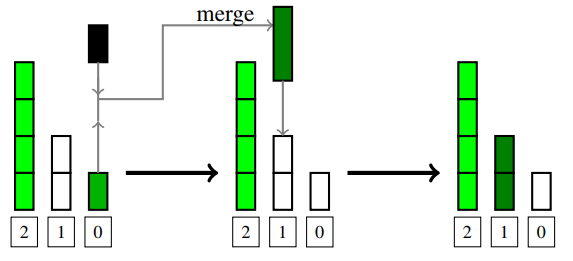
\includegraphics[width=0.75\linewidth]{Chapters/ParallelXFastTries/LSM.png} 
    \caption{Batch insertion with already 5 inserted batches - image extracted from Ashkiani et al.~\cite{ashkiani2017gpu}, arXiv:1707.05354}
\end{figure}

Let's first clarify that the different dictionaries\index{Dictionnary} used internally by this data structure have sizes that are powers of 2 and multiples of $b$ (i.e. $b2^{i}$). To insert or delete elements, we first sort the data related to the batch. Then, we always apply the same procedure, we check if the $i$th level is complete or empty (they cannot be partially filled), if it is empty, we insert all our elements. Otherwise, the elements to be inserted are merged with the elements of the $i$th level, the two containers become one and the previously filled level is emptied. We then try to insert the result in the next container, and so on until we find an empty dictionary\index{Dictionnary}. It should be noted that the filled levels correspond to the bit set to 1 in the binary representation of the number of batches inserted $r$, and 0 for the empty ones. There are thus $n = br$ elements in the structure. The total amount of work to insert $n$ elements is thus $O(rb \log r)$ since the worst case is complete cascading $O(rb)$ and this occurs with $O(i) \leq O(\log r)$. Observe that duplicates may exist naturally and that deletions correspond to sentinel values sharing the same key. In their implementation, they propose to set the most significant bit to 1 to indicate a deletion, which will serve in the merge procedure.

Queries can be simply implemented through classic lower/upper bound queries on each filled level and leading to natural $O(\log^{2} n)$. Note that merge procedures are somewhat difficult to implement in a parallel context, especially when duplicates exist~\cite{green2012gpu}.


\section{Implementation}

We will come back to some points linked to these data structures which seem for us important. In practice, LSMs\index{LSM} are way easier to implement than X-fast tries\index{X-fast trie}.

\subsection{X-fast trie}

We started by looking to see if there was any work on how to make x-fast tries\index{X-fast trie} concurrent\index{Concurrent} and we did not come across any results in this direction. So we tried to do what we could to solve the problem.

In practice, making the data structure concurrent\index{Concurrent} does not seem to be an impossible task even if it is somewhat difficult and much attention must be paid to it. We started by making ``atomic'' the internal nodes of the tree, i.e. if two threads try to insert the same node into the tree, the second will necessarily apply the procedure of merging (upsert) on the data it was in charge of and the one previously inserted. The merge procedure is the same as the node update procedure, atomically replaced in order to keep the key of the minimum and maximum element of the whole subtree.

Note that node updating plays a very important role in this concurrent\index{Concurrent} problem. Indeed, when one wishes to insert a node at the level of the leaves, one wants to have the smallest interval of values which exists and which contains the key of the new element. This avoids having to go through too many elements and therefore minimises the concurrency\index{Concurrent} problems there, by minimising the time spent there. The first step is to insert the element with its closest neighbors into the data structure. This avoids searching for an element that does not yet exist in the leaves but is described in the intermediate nodes.

Now all that remains is to correct it and update its neighbours to indicate its existence. The same procedure is always followed until the situation is resolved. The aim is to reduce the interval while it is possible. We update the predecessor and successor values of the node we want to insert. We make a ``compare and swap''\index{Compare and swap} on the previous node to put ourselves as successor, idem for the next one, we modify its predecessor. If both succeed, then we're done. Otherwise, the procedure is repeated again. Boundary and degenerate cases are limited by the fact that the structure provides the smallest interval ab initio.

\subsection{LSM\index{LSM}}

We tried to obtain the LSM\index{LSM} source code from the authors, who politely declined our request. We have therefore sought to replicate it based on the description made in their article which is nevertheless sufficiently clear and precise. We used the same two primitives to sort our data and merge dictionaries. And we hope we have provided an implementation that we feel is relatively fair and sufficiently close to what they have done. The structure being very simple, variations on possible implementations should be minor.

One of the key points of this structure is its inherent sequentiality\index{Sequential}. It seems difficult to propose a concurrent\index{Concurrent} version or, at least, to have something effective. We have to wait until the treatment between two levels is completely done before we can do anything else. As there are also very few levels in the structure, a very huge contention will be observed on the first levels making it essentially serialized. It was also easier to use two buffers to merge our data, as suggested in the original paper. So we work on a single block and on only 16 warps out of 32 available. Indeed, the library we use to sort requires some ``shared'' space (linked to a block) that we did not have enough to support 32 warps per block.


\section{Experiments}\label{PARALLELXFASTTRIERESULTS}

For the experiments, we have again put in place a simple experimental protocol. We tested the three canonical operations: insertion, search and predecessor query, the ones that interest us the most, we can expect an equivalent time for successor or deletion requests. We compared the performance obtained for three different data structures, X-fast tries\index{X-fast trie}, B-trees and LSM\index{LSM}; each under special conditions.

For the insertions, the B-trees\index{B-tree} have no concurrent\index{Concurrent} version known as being really effective, we therefore reused the data structure developed in the chapter relating to X-fast tries$^{[\ref{BTREE}]}$ and this in a sequential\index{Sequential} context, i.e. with only one warp in only one block.

For LSM\index{LSM}, the situation is different, first, it is difficult to provide true parallelism to this data structure given its inherent sequentiality\index{Sequential} and, second, for technical reasons, we have not been able to launch more than 16 warps related to too much shared memory use for the sort primitive used.

Finally, for the X-fast tries, the problem was quite different, crashes appeared in some rare case. Of course, we investigated the reasons for these problems, but the bugs did not seem obvious to us. Nonetheless, we have been able to carry out a sufficient number of experiments and we may hope that the results would be representative of those actually obtained.

On the other hand, for queries, there is no reason to deprive ourselves of the parallelism offered by graphics cards\index{Graphics cards}, so we decided to use 16 warps and 32 blocks, which should be enough to saturate the streaming processors and therefore get the maximum theoretical performance. All tests were performed with pre-allocated memory and the hash tables\index{Hash table} had a capacity equal to twice the expected number of elements, thus a load factor of 50\%. We collected the results on 20 runs and 5 iterations.

\section{Results}

As usual, we will present each of the experiments that were conducted associated with its relative conclusions. The size of the points represents the standard deviation obtained in the results and their position the mean value.

We'll start with the insertions and we can observe several phenomena:

\begin{figure}[!htb]
    \centering
    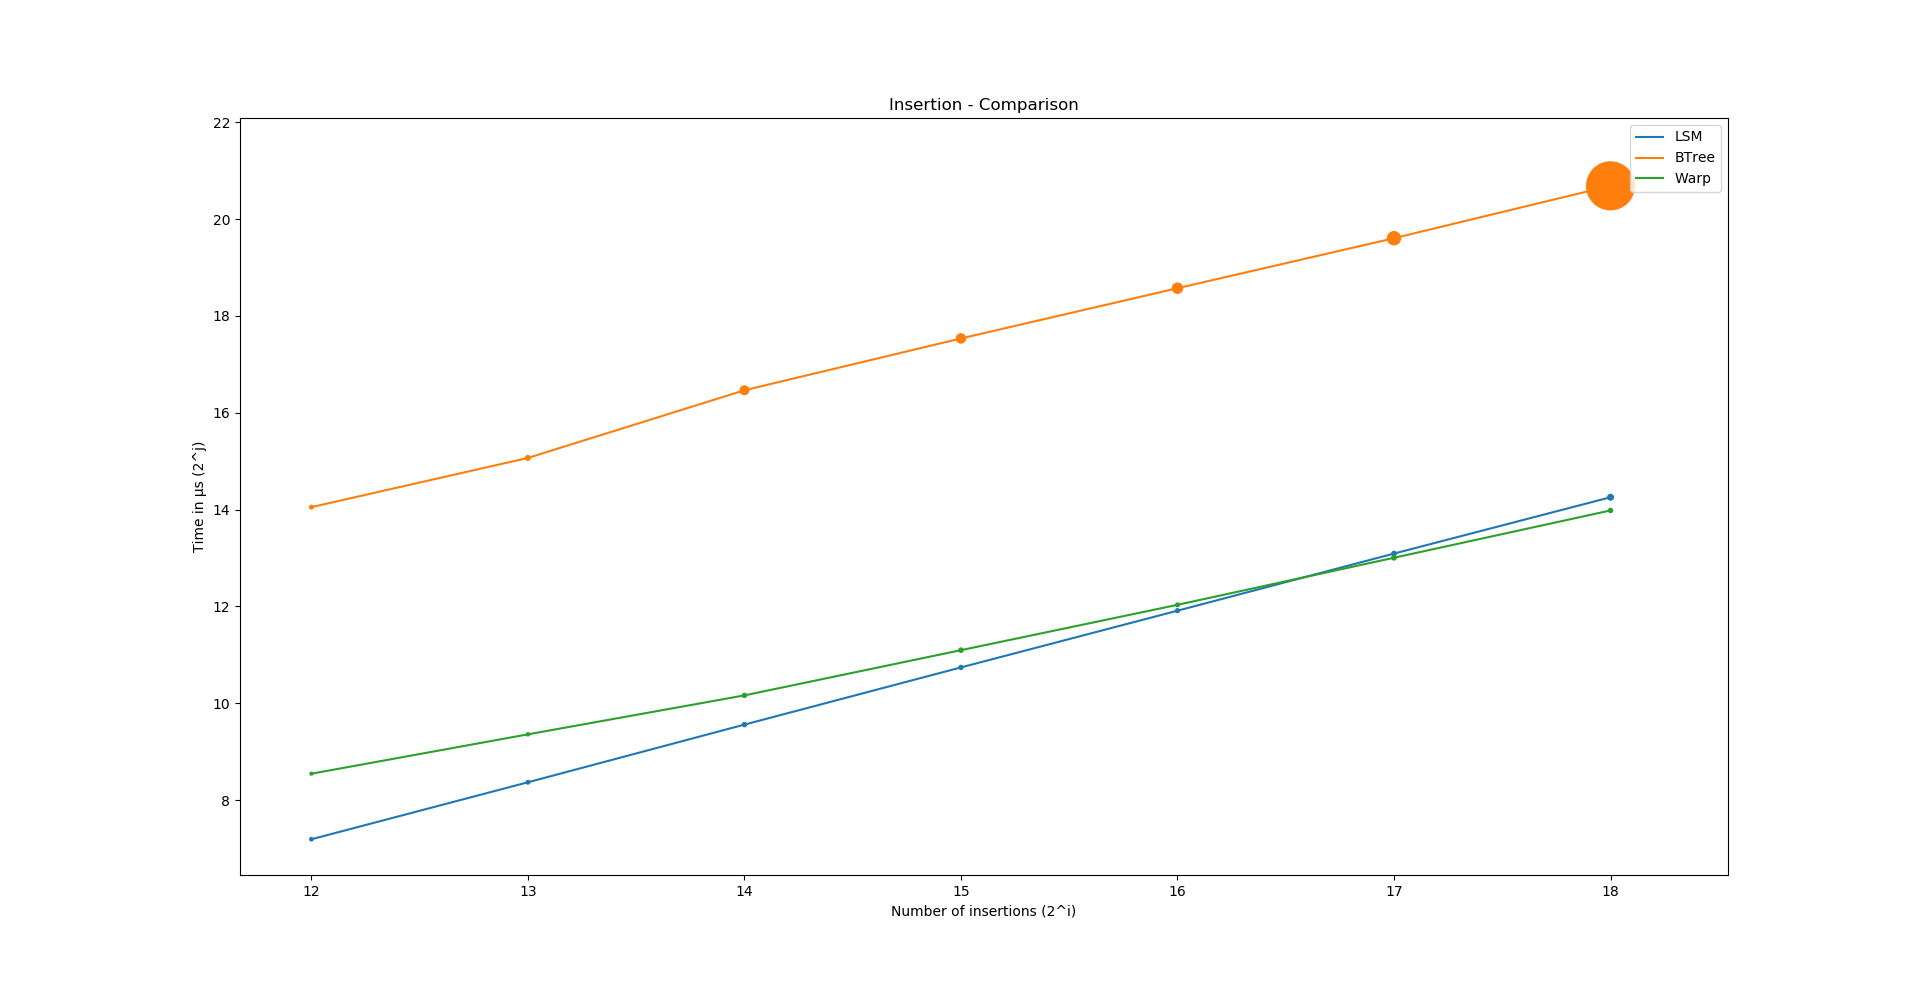
\includegraphics[width=\linewidth]{Chapters/ParallelXFastTries/Insertions.png} 
    \caption{32-bit key insertion}
\end{figure}

\begin{itemize}
    \item The standard deviation is a bit lower for X-fast tries\index{X-fast trie}. Indeed, it seems relatively clear that their variance is only dependent on the queries performed on the internal hash tables\index{Hash table}. But the load factor is relatively low, only 50\%, so it seems normal to have a narrow variance. On the contrary, we had already observed that the B-trees\index{B-tree} had a stronger tendency to have high variances related to the rebalancing necessary to maintain the structure in the tree. Finally, the LSM\index{LSM} have an associated variance relatively small in comparison to that of the B-trees\index{B-tree}, this is related to the cascading merge which must be carried out each time one passes to the next power of 2.
    \item The gain in concurrency that we have obtained by exploiting more warps for X-fast tries\index{X-fast trie} is very interesting. For both LSM\index{LSM} and X-fast tries\index{X-fast trie}, insertions are almost 100 times faster than for sequential B-trees\index{B-tree}.
    \item The LSM\index{LSM} offers lower starting constants but the coefficients of the larger orders seem larger. This does not seem so irrelevant since the merge operation is not totally without cost (the cost to sort the original buffer remains marginal~\cite{ashkiani2017parallel}). The LSM primitives are incredibly fast but the cascading mecanism remains significant on the performances.
    \item In this context, insertions in X-fast tries\index{X-fast trie} seem to be a good alternative to LSM\index{LSM}, following the batch size used of 512; and with greater flexibility, element-wise and not like in a bulk synchronous model. Note that the batch size presented in the original article was quite different, by a factor of more than 32 and that our implementation is not as optimal as their one.
\end{itemize}

We will continue with the two search operations:

We will start with thread-based queries:

\begin{figure}[!htb]
    \centering
    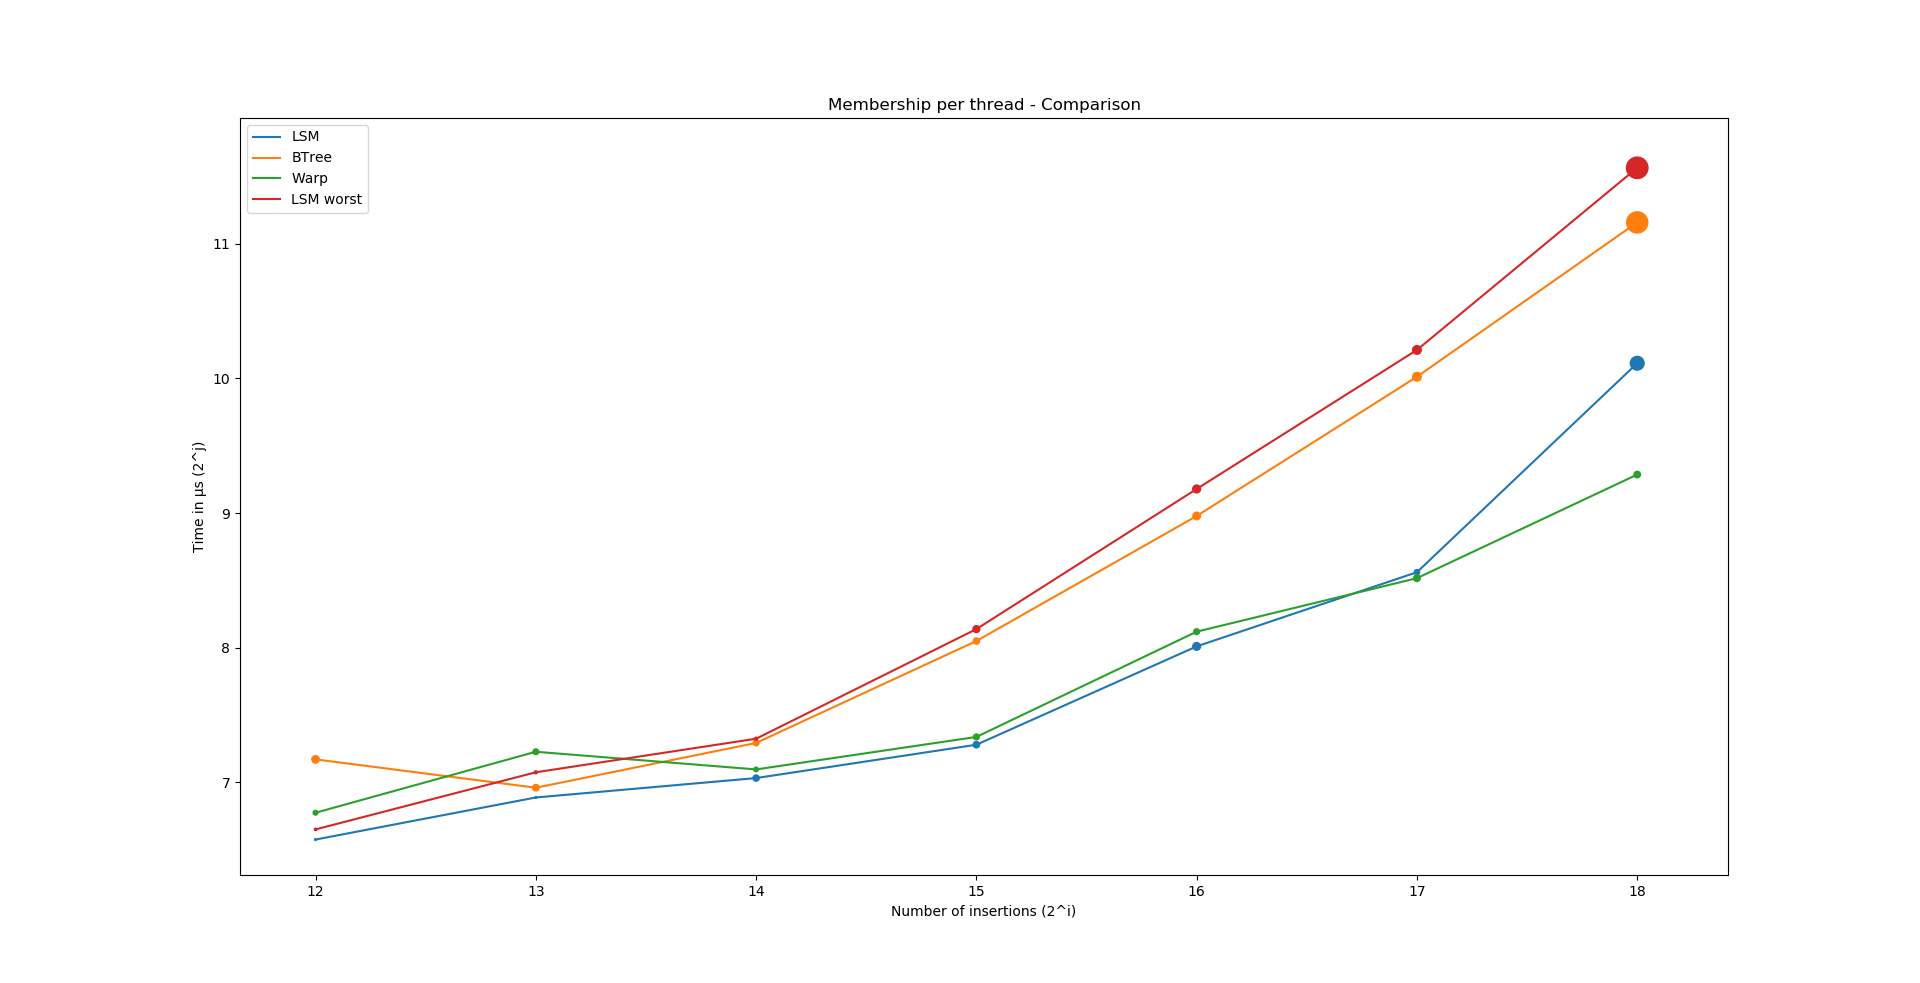
\includegraphics[width=0.85\linewidth]{Chapters/ParallelXFastTries/Membership_thread.png} 
    \caption{Thread-based searches}
\end{figure}

The results are somewhat astonishing:
\begin{itemize}
    \item Very logically, accessing X-fast tries\index{X-fast trie} elements is faster than for B-trees\index{B-tree}, since it consists of a simple search in a hash table\index{Hash table}, instead of running through an entire tree.
    \item But the difference between X-fast tries\index{X-fast trie} and LSM\index{LSM} is very surprising, they are really close. The main argument is related to the fact that the locality of the data is much stronger in the LSM\index{LSM}. The first pivots used during the dichotomous search, have strong chances to be kept in memory since they will be very often requested. We are also in the ideal situation for LSM where only one dichotomous search must be performed, since we have inserted a power of 2 elements ($b2^{k}$).
    \item When requests are made in the worst case for LSM, which corresponds to a number of insertions which is a power of 2 minus 1 ($b2^{k} - b$), the performances become comparable to that of a B-tree due to the potential $O(\log N)$ queries made. On average, the LSM remains better than the B-tree.
\end{itemize}

Now, the warp-based queries where the whole warp contributes to search one element:

\begin{figure}[!htb]
    \centering
    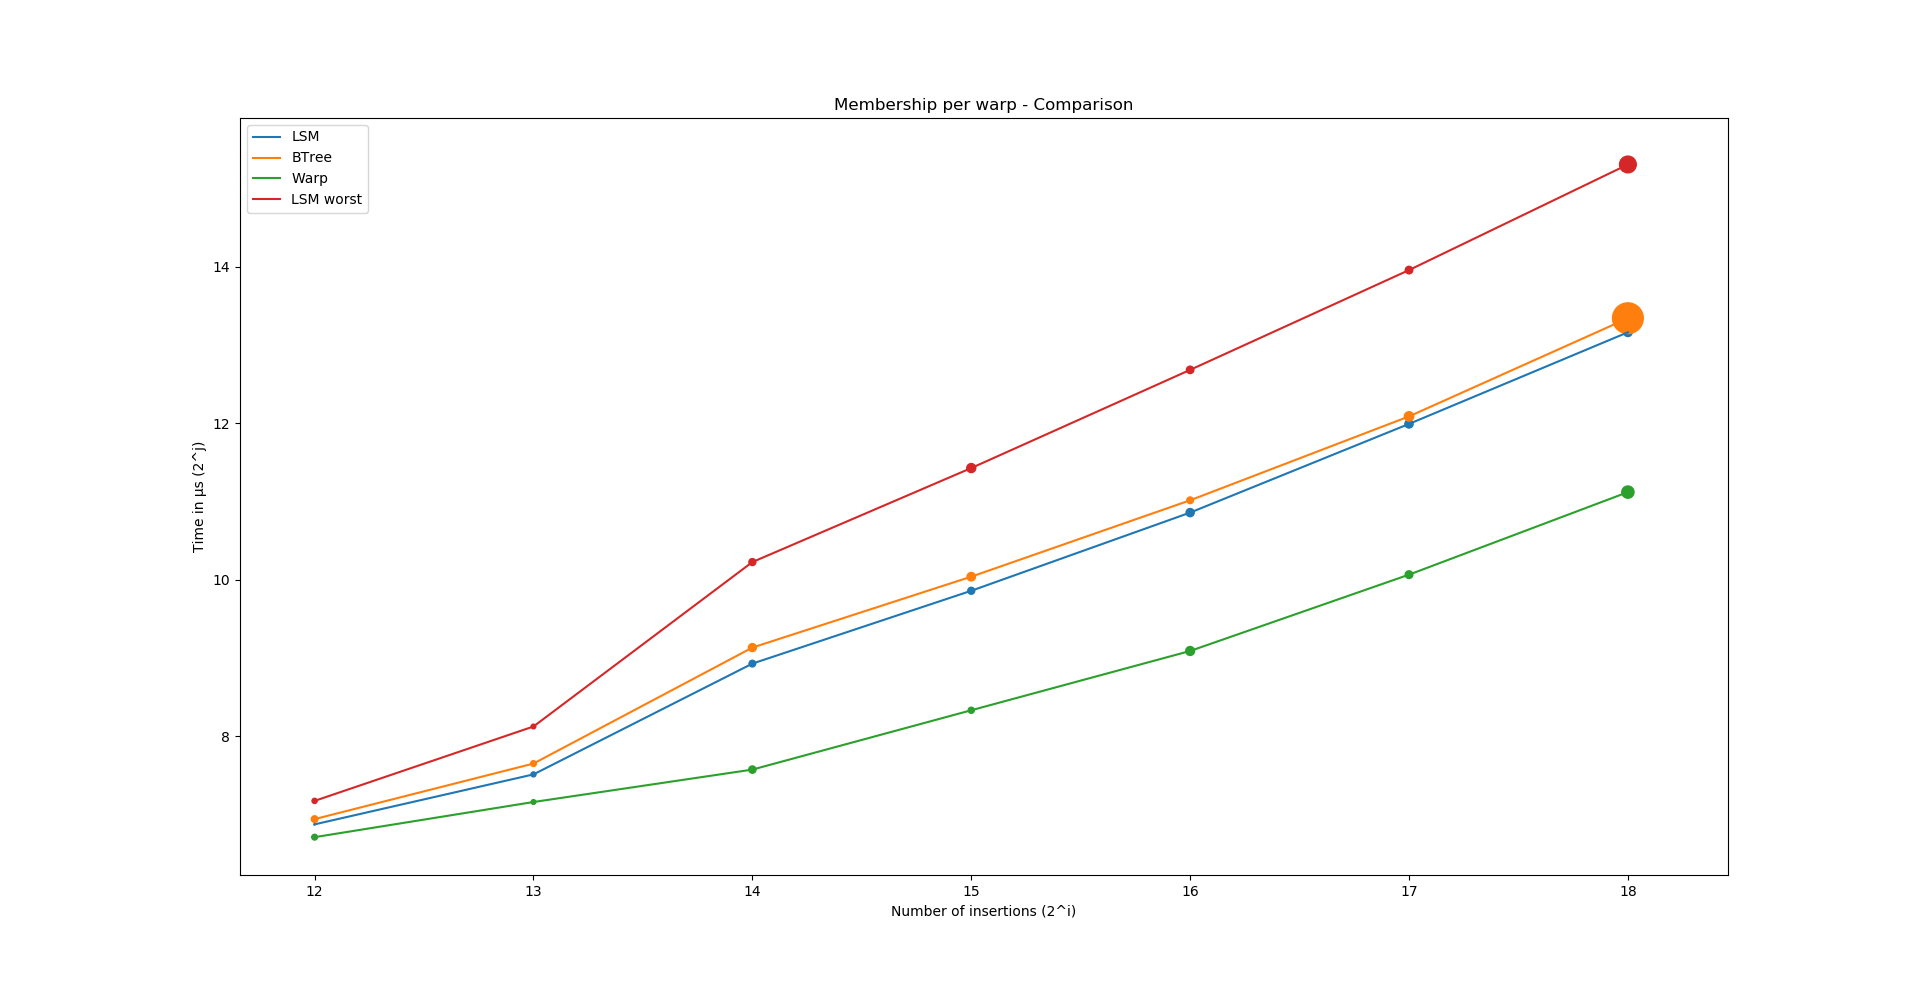
\includegraphics[width=0.85\linewidth]{Chapters/ParallelXFastTries/Membership_warp.png} 
    \caption{Warp-based searches}
\end{figure}

We observe similar phenomena:
\begin{itemize}
    \item The best case for LSM\index{LSM} is close to B-trees because dichotomous key searches no longer have to be performed. So all that remains is the cost of searching properly and loading the different blocks.
    \item X-fast tries\index{X-fast trie} retain their advantage thanks to the multiple probes performed at the same time in the leaf-level hash table\index{Hash table}.
\end{itemize}

\newpage

Finally, all we have left to observe are the predecessor's queries:

\begin{figure}[!htb]
    \centering
    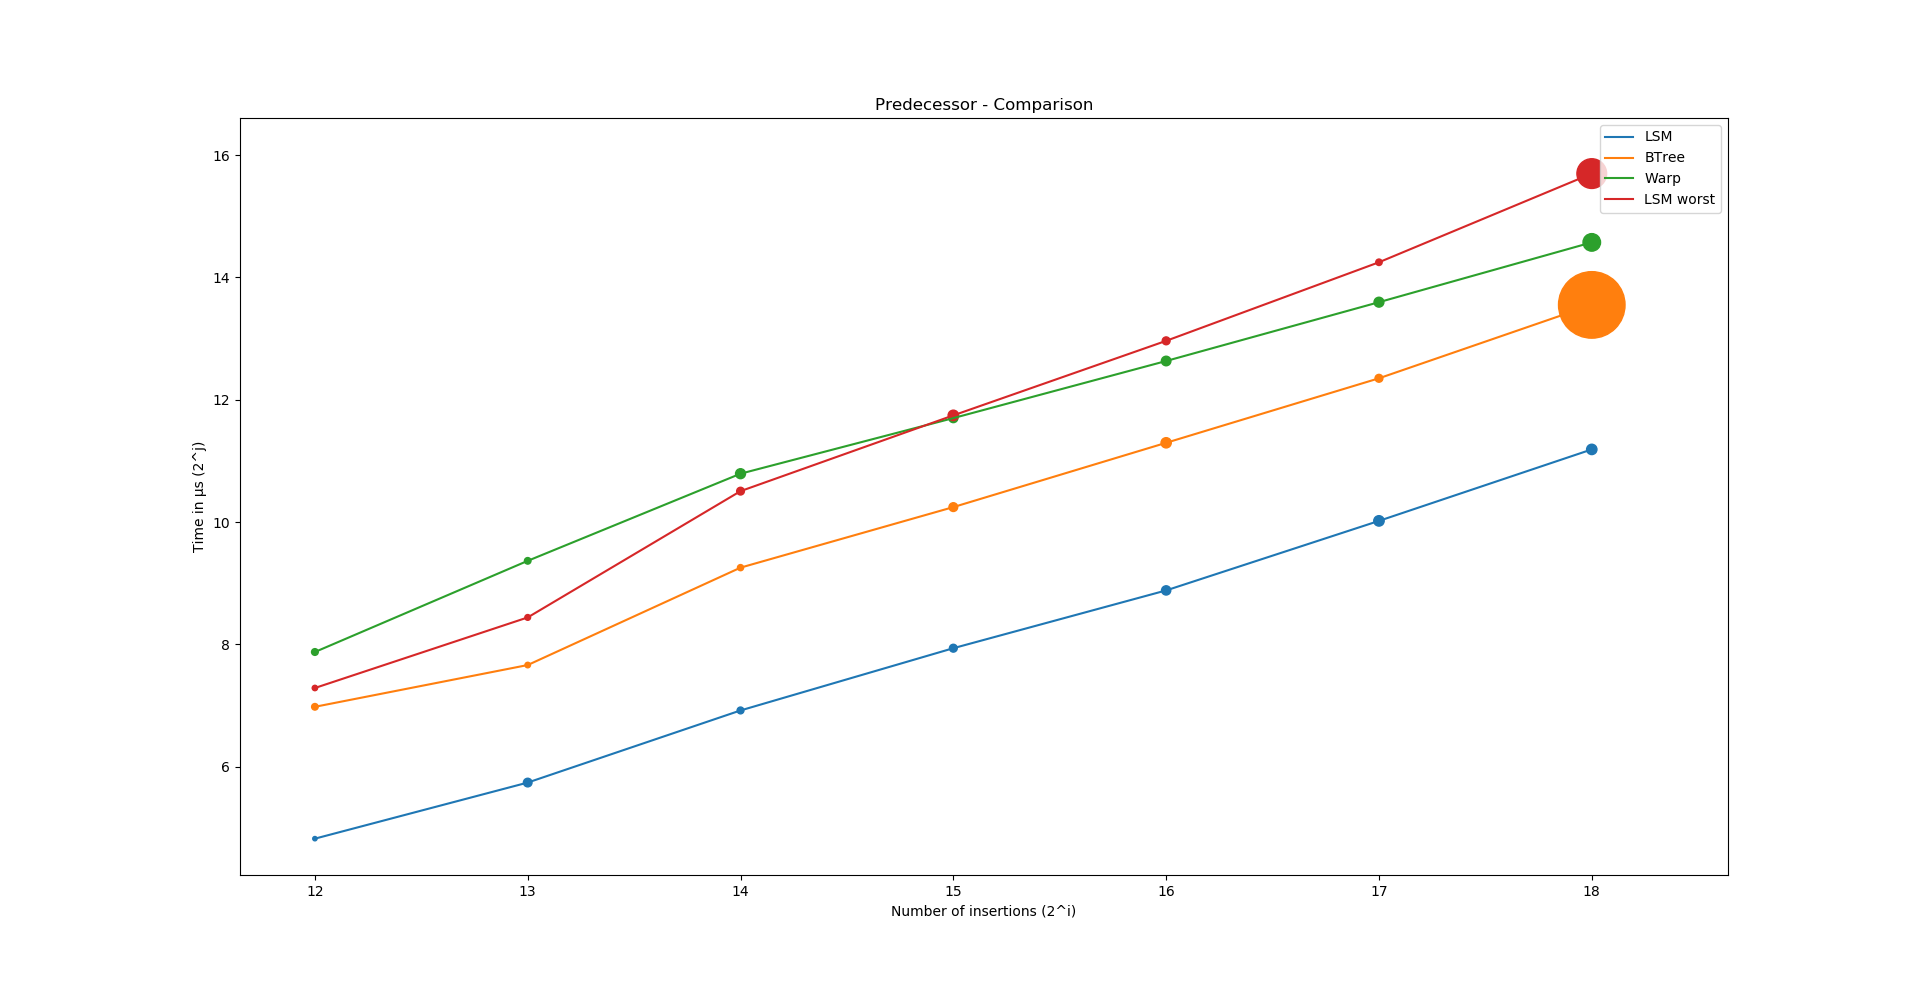
\includegraphics[width=\linewidth]{Chapters/ParallelXFastTries/Predecessor.png} 
    \caption{Warp-based predecessor queries}
\end{figure}

Some remarks can be made:
\begin{itemize}
    \item We notice the same phenomenon as in the sequential\index{Sequential} framework, X-fast tries\index{X-fast trie} are slower than B-trees\index{B-tree} because of their imposing number of memory requests.
    \item For the LSM\index{LSM}, the performance is roughly equivalent to the search operation, which is quite logical since both use lower bound algorithm.
    \item We precise that the predecessor search can be done by thread for LSM, whereas for X-fast tries, it can only be done by warp. So we simulated this operation by performing only one of the queries in the warp to make it comparable to other data structures.
    \item De facto, the time that would be taken to search for the predecessor per thread for LSM\index{LSM} would be even faster than pseudo warp-based, and a gain of a factor 8 would not seem excessive.
    \item Predecessor requests in X-fast tries are faster than those in a LSM in the worst case, but on average they are significantly slower.
\end{itemize}



\section{Speed-up}

After collecting all these data and results, we asked ourselves what was the scalability of such a data structure. And mainly, what was the influence of the number of blocks and warps on the performances. Indeed, with material advances, we can expect an increase in these resources both in quantity and in speed (cost related to latency, scheduling,...). Will it remain interesting in a more distant future.

So we collected data on the insertion of 131 thousand items ($2^{17}$) for many configurations. We varied the number of blocks and warps from 1 to 32 and from 1 to 16 respectively by doubling each time their number. We present the mean time associated with its standard deviation (in parenthesis). The intermediate lines represent the ratio between the time taken for that specific configuration and that with only one block and one warp (and therefore non-concurrent).

\begin{table}[]
\centering
\caption{Time to insert 32-bit keys in function of the number of warps and blocks}
\label{my-label}
\resizebox{\textwidth}{!}{
\begin{tabular}{ccccccc}
         & \# Warps 1           & 2                    & 4                    & 8                   & 16                 \\
\#Blocks &                      &                      &                      &                     &                    \\
1        & 611080.18 (2151.349) & 306842.126 (970.405) & 154465.447 (203.045) & 80001.789 (163.276) & 42918.908 (81.063) \\
         & 100.0                & 50.21                & 25.28                & 13.09               & 7.02               \\
2        & 316926.742 (789.772) & 159116.154 (579.524) & 80069.378 (101.706)  & 41476.388 (98.77)   & 22452.94 (44.331)  \\
         & 51.86                & 26.04                & 13.1                 & 6.79                & 3.67               \\
4        & 160547.17 (356.854)  & 80964.003 (269.402)  & 40692.377 (88.208)   & 21198.831 (38.379)  & 11562.582 (31.429) \\
         & 26.27                & 13.25                & 6.66                 & 3.47                & 1.89               \\
8        & 81903.641 (182.339)  & 41682.092 (131.041)  & 21026.405 (63.426)   & 11649.702 (36.151)  & 7061.199 (49.369)  \\
         & 13.4                 & 6.82                 & 3.44                 & 1.91                & 1.16               \\
16       & 41745.251 (124.893)  & 21266.58 (90.145)    & 11281.267 (51.34)    & 6674.541 (30.823)   & 7487.541 (43.459)  \\
         & 6.83                 & 3.48                 & 1.85                 & 1.09                & 1.23               \\
32       & 21303.918 (62.376)   & 11469.453 (34.3)     & 6597.327 (17.209)    & 7461.54 (32.463)    & 5709.916 (33.266)  \\
         & 3.49                 & 1.88                 & 1.08                 & 1.22                & 0.93                 
\end{tabular}
}
\end{table}

The results are self-explanatory:
\begin{itemize}
    \item Generally speaking, we see the times reduced with the increase in parallelism capacities.
    \item The times are roughly equivalent on the diagonals, which is relatively logical. And implies that both the increase in the number of blocks and warps contribute to the overall performance improvement.
    \item The speed-up is far from being linear, we get more than 20\% of variation from the theoretical increase for configurations such as $\#warps \times \#blocks \geq 128$. And we're almost at a factor $2$ on the last configuration proposed where we reach nearly the maximum possible speed. This may be explained by the fact that we are beginning to reach the maximum possible bandwidth and that the concurrency problems on the double-linked list at the leaf level are not totally without cost.
\end{itemize}




\section{Interleaved operations}

Finally, we would like to point out that we have only considered bulk operations, where only one type of operation is carried out. This case is obviously very far from reality where a mixture is by no means exceptional. We would therefore like to come back to this point.

We clearly expect that interleaving operations and proving that implementations are correct will not be an easy task. Some mixtures don't seem to pose much of a problem at first glance. Indeed, all those who look for an element in the structure correspond to the classic case of hash tables, hence, we have the standard guarantees. Inserting elements and searching for a predecessor/successor doesn't seem too difficult either if you allow yourself a certain flexibility on the results you want to obtain.

The real concerns come with the removal of elements. Indeed, both at the level of the leaves and the maintenance of the sorted list and at the levels of the intermediate leaves and the maximum/minimum values of the subtree, problems can arise. Perhaps invalidating elements and rebuilding the structure from time to time would be a better solution.


\section{Conclusions}

As we have seen, the results we obtained in the sequential\index{Sequential} framework are surprising close from those obtained in the concurrent\index{Concurrent} framework. Of course, we expected a certain loss of performance related to the very large number of memory accesses needed to respond to requests, unlike the very limited subset proposed by the LSM\index{LSM}, but clearly not in such measures.

The theoretical performance offered by X-fast tries\index{X-fast trie} was really important to check and adapt to the context of the graphics cards\index{Graphics cards}. This data structure proposes a real alternative to LSM. We want to emphasize that we are far from the number of insertions being announced in their article since we used smaller batch sizes, but our data structure has the advantage of offering insertions by element.

One of the big black spots of this data structure is obviously the need to abuse atomic\index{Atomic} operations, and these are inherently terribly slow. We count no less than 7 million atomic transactions to insert a hundred thousand elements, however the system can provide more than 7GB/s for these operations. Nonetheless, the performances remain interesting. The other one is the amount of memory needed to hold the structure in memory which is incredibly huge. We stopped our experiments for more than 250 thousands ($2^{18}$) of insertions since we reach the limits of our available memory.

To resume, we achieve equivalent performance for insertions (10Mop/s) and thread-based searches (300Mop/s). We are faster on searches that use an entire warp (110Mop/s vs 30Mop/s) and we are slower on average on predecessor queries (10Mop/s vs 30Mop/s). Our data structure is of interest if the number of predecessor/successor requests remains lower than the search operations.

Nevertheless, we obtained these results in an ideal case, where all the space had been pre-allocated. One expects to become notoriously slower on insertions in practice. The load factor used in hash tables is relatively low 50\%, one can also lose efficiency there.

Besides, it has the advantage of being able to improve itself thanks to scientific or material advances. It also explores a path in research where parallelism can be used at lower cost to find elements effectively. We can hope to see other more advanced structures employing similar techniques, like warp election.

To conclude, we have tried to group in a single table the main differences proposed for the only two existing dynamic dictionaries\index{Dictionnary} on GPUs\index{Graphics cards}, at this time, in order to have a more theoretical and high level aspect of what is proposed in practice.

\newpage

\begin{table}[!htb]
\centering
\caption{Resume comparison of LSM\index{LSM} and X-Fast tries}
\label{my-label}
\begin{tabular}{ccc}
                     & LSM                  & X-Fast tries          \\
Insertion            & Bulk and Block       & Element and Warp       \\
$w = |\text{warp size}|$ & $O(\log N)$          & $O(\frac{\log u}{w})$ \\
\multicolumn{1}{l}{} & \multicolumn{1}{l}{} & \multicolumn{1}{l}{}  \\
Search               & Thread               & Thread                \\
                     & $O(\log^{2} N)$      & $O(1)$                \\
\multicolumn{1}{l}{} & \multicolumn{1}{l}{} & \multicolumn{1}{l}{}  \\
Predecessor          & Thread               & Warp                  \\
                     & $O(\log^{2} N)$      & $O(\frac{\log u}{w})$ \\
\multicolumn{1}{l}{} & \multicolumn{1}{l}{} & \multicolumn{1}{l}{}  \\
Range queries        & Yes                  & No\footnotemark       \\
$L$ output           & $O(\log^{2} N + L)$  & $O(L)$                \\
\multicolumn{1}{l}{} & \multicolumn{1}{l}{} & \multicolumn{1}{l}{}  \\
Concurrency          & Difficult            & Medium                \\
Memory               & Proportional (3N)    & Huge (+100N)$^{2}$    \\
Variance             & High                 & Small                 \\
Requirements         & Comparable keys      & Only integers         \\
Implementation       & Easy                 & Hard          
\end{tabular}
\end{table}
\footnotetext{Lazy iteration on the elements.\\$~\quad~^{2}$Proportional to $\Theta(3 N \log u)$.}

% TALK ABOUT LINEARIZABILITY


%http://people.cs.georgetown.edu/~jfineman/papers/cobtree.pdf
%Correctness
%We first argue that the data structure is correct, even under concurrent
%operations. The most common way of showing that an algorithm
%implements a linearizable object is to show that in every
%2The hyperceiling of x, denoted ddxee, is defined to be 2
%dlogxe
%, i.e.,
%the smallest power of 2 greater than x.
%execution there exists a total ordering of the operations with the
%following properties: (1) the ordering is consistent with the desired
%insert/search semantics, and (2) if one operation completes before
%another begins, then the first operation precedes the second in the
%ordering. Linearizability follows due to a straightforward extension
%of Lemmas 13.10 and 13.16 in [22].